%!TEX root = ../../../super_main.tex

\section{Collaboration with Group SW613F15}
\label{sec:collaboration_with_group_sw613f15}

After the recent handover of \gc from group \emph{SW604F15} (us) to \emph{SW613F15}, it was discovered that a component in \ps (developed by \emph{SW613F15}) was not consistent with the design implemented in the \launcher (implemented by \emph{SW604F15}) regarding showing of multiple items, applications and pictograms respectively. This inconsistency can be seen in \figref{fig:collab_with_group_13}.

\begin{figure}[!htbp]
    \centering

    \begin{subfigure}[t]{0.75\textwidth}
        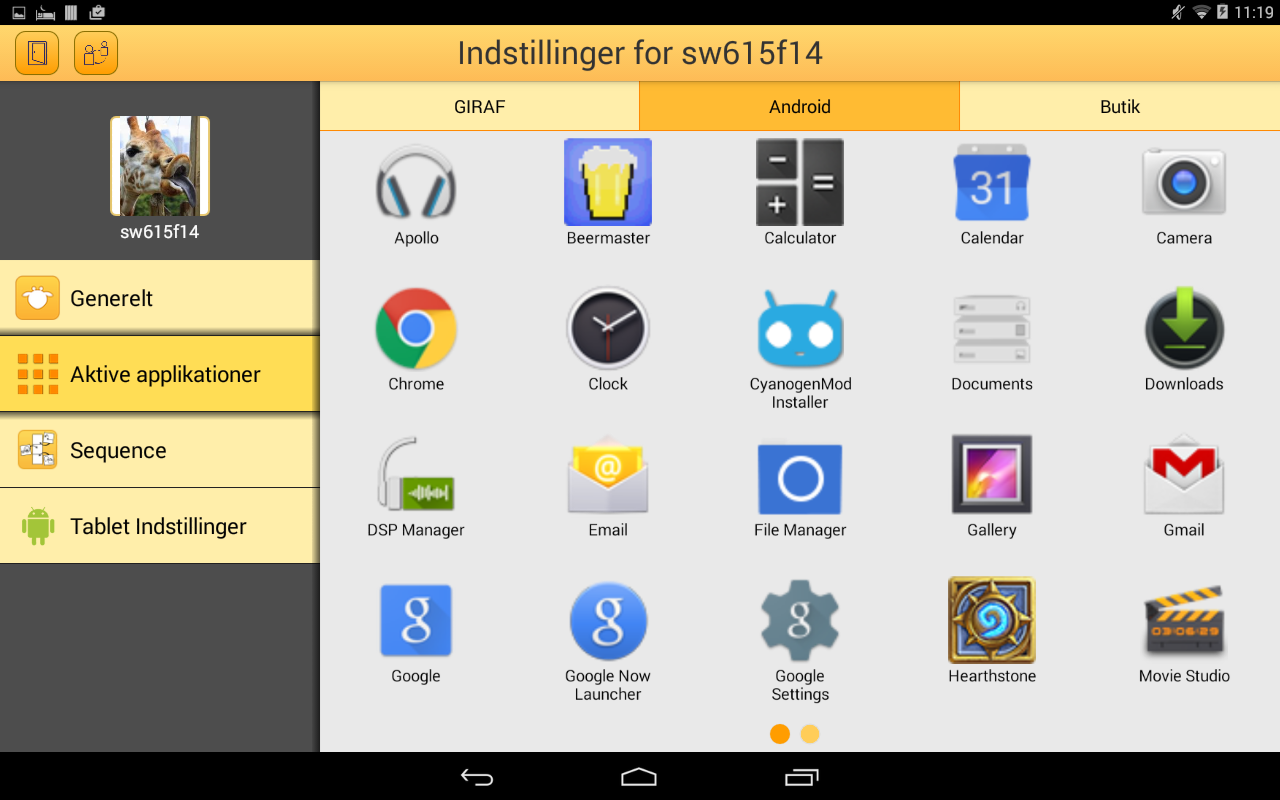
\includegraphics[width=\textwidth]{sprint_three/collab_with_group_13/launcher.png}
        \caption{Launcher}
        \label{fig:collab_with_group_13_launhcer}
        \vspace*{1cm}
    \end{subfigure}
    \hfill
    \begin{subfigure}[t]{0.75\textwidth}
        \includegraphics[width=\textwidth]{sprint_three/collab_with_group_13/pictosearch.png}
        \caption{Old \ps}
        \label{fig:collab_with_group_13_pictosearch}
    \end{subfigure}
    
    \caption{Problem visualized}
    \label{fig:collab_with_group_13}
\end{figure}

Since \emph{SW604F15} had already spent some time on implementing a viewpager for this purpose, a solution for \ps was made in collaboration by these groups. A slight implementation difference was that the viewpager in the launcher is implementing using a \androidinline{FragmentAdapter}, whereas the viewpager in \ps is implemented using \androidinline{GridView}s. This soloution was though found to be inconsistent in regards to the other displays of pictograms and it was decided that there should be distinction between how applications should be presented and how pictograms and profile pictures should be presented. For this reasons we assisted \emph{SW613F15} to implemented a \androidinline{GridView} like the one implemented in \ct. The final result of \ps can be seen in \figref{fig:pictosearch}.


\begin{figure}[!htbp]
    \centering
    \includegraphics[width=\textwidth]{sprint_three/pictosearch}
    \caption{\ps}
    \label{fig:pictosearch}
\end{figure}